% questions.tex —— 1977 年·广西百色卷（文科） · 题目内容片段（无答案）
% 由 tools/generate_projects.py 依来源总账自 1977/1977_数学真题_广西百色文_试题.md 生成，勿手改（改源 MD 后重跑）


\gkpart{广西百色试点（文科）}

\begin{gktip}
\textbf{来源说明}：本题面依据固定源 PDF《1977广西百色文》第 1—4 页（书页 147—150）逐题转录。固定源是题面与解答连排的书籍材料：每题题面后紧跟「解」「证法」，并非空白试卷；本文只转录题面，配套答案与解析由本库对照源解答独立复算推导，\textbf{非官方标准答案}。原卷按大题「一、」至「六、」编号，其中第一大题下有 4 个小题、第二大题下有 2 个小题；本库将大题重排为连续题号 1—6，大题内小题统一为（1）（2）…小问格式，未增删题干。原卷未标分值，无附加题、参考题。第 1 页顶部约有一行半被墨渍覆盖的文字（疑为书眉），无法辨认，未转录。
\end{gktip}

\par\medskip

\begin{question}
\gkti{1}

\Needspace{5\baselineskip}
（1） 计算：

\nopagebreak[4]
\[
-3.5-\left[2\frac{3}{7}-\left(-3\frac{3}{14}-3\frac{5}{14}\right)\right]
\]

（2） 当 $|m|=|n|$ 时，能肯定 $m=n$ 吗？为什么？

（3） 当 $a=1\frac{1}{2}$ 时，求 $a+\dfrac{1-2a+a^2}{a-1}$ 的值。

（4） 已知 $\log_x32=5$。求 $x$。

\end{question}
\begin{question}
\gkti{2}分解下列各式的因式：

（1） $(x-2)(x^2-3)+(x-2)^2-(x-2)(2x-3)$

（2） $bc^2+a^2c+ab^2-a^2b-ac^2-b^2c$

\Needspace{0.4\textheight}
\end{question}
\begin{question}
\gkti{3}已知 $AD$ 和 $BE$ 分别是 $\triangle ABC$ 的 $BC$ 和 $Ac$ 边上的高，延长 $AD$ 交外接圆于 $F$，求证 $\angle EBC=\angle FBC$。

\begin{gktip}
\textbf{源注}：源卷把边名 $AC$ 的第二个字母误排为小写「c」（印作 $Ac$），系排印之误；此处保留转录，应读作 $AC$。
原源 PDF 第 3 页在第三题证法二旁附有三角形与外接圆示意图；LaTeX 版按源图重绘。
\end{gktip}
\nopagebreak[4]
\begin{center}% 1977 年广西百色卷（文科）第 3 题：圆内接三角形 ABC，AD、BE 分别为 BC、AC 边上的高，
% AD 延长交外接圆于 F，虚线 DF、BF（按源卷第 3 页布局：A 左上、B 左、C 右、F 底部，E 在 AC 上近 A，D 在 BC 上）
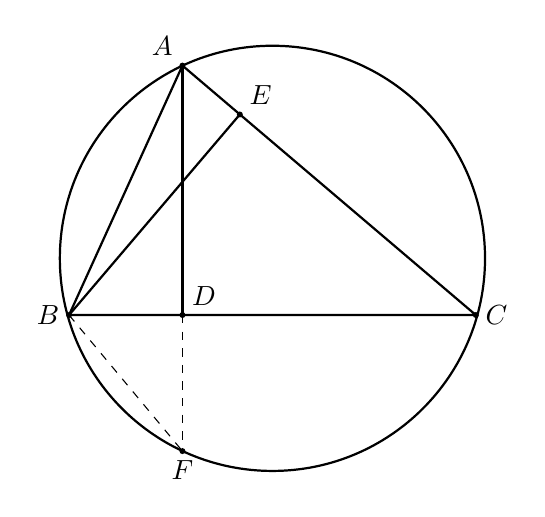
\begin{tikzpicture}[scale=0.9]
  \draw[thick] (0,0) circle (3);
  \coordinate (A) at (-1.27,2.72);
  \coordinate (B) at (-2.87,-0.8);
  \coordinate (C) at (2.87,-0.8);
  \coordinate (D) at (-1.27,-0.8);
  \coordinate (E) at (-0.46,2.03);
  \coordinate (F) at (-1.27,-2.72);
  \draw[thick] (A)--(B)--(C)--cycle;
  \draw[thick] (B)--(E);
  \draw[thick] (A)--(D);
  \draw[dashed] (D)--(F);
  \draw[dashed] (B)--(F);
  \fill (A) circle (1.2pt) node[above left] {$A$};
  \fill (B) circle (1.2pt) node[left] {$B$};
  \fill (C) circle (1.2pt) node[right] {$C$};
  \fill (D) circle (1.2pt) node[above right] {$D$};
  \fill (E) circle (1.2pt) node[above right] {$E$};
  \fill (F) circle (1.2pt) node[below] {$F$};
\end{tikzpicture}
\end{center}
\nopagebreak[4]
\end{question}
\begin{question}
\gkti{4}红星农场一块地，用一台拖拉机来耕 $6$ 天，完成一半，后来加入了另一台新式拖拉机，两台合耕两天就耕完余下的地，新式拖拉机单独耕这块地要几天？

\end{question}
\begin{question}
\gkti{5}曙光人民公社养鸡场，准备在鸡舍后面开辟一个矩形养鸡场，现仓库里有 $38$ 米长的铁丝网，问鸡场的长和宽各是多少米？才能使鸡场的面积最大？（靠鸡舍一边不围网）

\end{question}
\begin{question}
\gkti{6}已知一个动点 $P(x,y)$ 到两定点 $A(1,3)$ 和 $B(-3,5)$ 的距离相等，求这动点的轨迹方程。

\end{question}